\chapter{Introdução}
\label{cap:introducao}

Atualmente, as crianças e jovens brasileiros possuem cada vez mais acesso e contato
com tecnologias digitais. Cerca de 75% dos jovens entre 10 e 18 anos afirmam navegar
na internet, e destes 38,3% afirmam utilizar este acesso para estudos e realização de tarefas
escolares (PALOSCHI, 2012). Alem disso, de acordo com o Horizon Report (JOHNSON;
ADAMS; CUMMINS, 2012), mundialmente, as instituições de ensino aumentam cada vez
mais a disponibilidade e a qualidade de acesso a internet dentro de suas dependências.

Os estudantes também trazem cada vez mais seus próprios dispositivos para as salas de
aula (Bring Your Own Device (BYOD), como notebooks, tablets e smartphones, dispositivos
estes que também são utilizados para seus estudos fora de sala de aula. Dessa forma,
esses dispositivos podem enriquecer o aprendizado em diversos lugares e momentos, e não
somente nas salas de aula (JOHNSON et al., 2014). Este ambiente propício, vem abrindo espaço para a utilização de aplicativos e sistemas computacionais educacionais para aumentar a eficiência da atividade de ensino e aprendizagem. 

Os sistemas educacionais vem evoluindo juntamente com a computação, e tem como objetivo servir como meio ou ferramenta para contribuir objetivos pedagógicos (Pierre Tchounikine), e a informática na educação vem evoluindo entre vários aspectos, entre eles, com o objetivo de servir realmente como um meio de instrução, como na educação mediada/assistida por computadores, através do uso de tutores inteligentes, melhorando a forma de avaliação de desempenho dos alunos, influenciando e gerando interesse e motivação, possibilitando o uso de metodologias pedagógicas antes impraticáveis sem a computação, o uso de dispositivos móveis e redes sociais.

Os sitemas computacionais para educação também podem variar de acordo com o objetivo a que se destina. Há no mercado sistemas que ajudam no processo de ensino e aprendizagem, outros que servem de tutores inteligentes, e também sistemas que ajudam a escola a gerenciar outros aspectos relacionados ao processo, como a performance do aluno. Os sistemas computacionais para educação além de 

computer assisted instruction, 
tutores inteligentes
melhorar o desempenho dos alunos em exames de qualificação padronizados (lembrar de TRI e Bloom, 1984
influenciar motivação e interesse (Raines e Clark, 2011 e aqueles artigos de geração de rede)
metodologias impossíveis sem computação
dispositivos moveis
redes sociais

Neste contexto, foram elaboradas as seguintes perguntas de pesquisa para este trabalho:

\textbf{Pergunta 1:} quais seriam as funcionalidades interessantes a um possível sistema colaborativo a ser utilizado dentro e fora de sala de aula?

\textbf{Pergunta 2:} considerando estes requisitos e considerando que o sistema possa ser utilizado em várias plataformas e dispositivos, quais as tecnologias seriam adequadas a seu desenvolvimento?

Com base nas perguntas de pesquisa definidas anteriormente, chega-se ao objetivo principal deste trabalho, que é o levantamento das funcionalidades interessantes a um sistema colaborativo a ser utilizado dentro e fora de sala de aula, a pesquisa das tecnologias indicadas ao seu desenvolvimento. Adicionalmente, será avaliado o sistema como um todo através de um experimento prático em sala de aula.

\section{Organização do documento}

Nesta introdução foi definido contexto, as perguntas de pesquisa e o objetivo geral e secundários do trabalho. E também pontuou a estrutura deste documento.

No Capítulo 2 é apresentado a fundamentação teórica, onde são definidos e contextualizados os conceitos relacionados a este trabalho, como: aprendizado colaborativo, sistemas de informação educacionais, colaboração, etc. Já o Capíitulo 3,....


\chapter{Fundamentação}
\label{cap:fundamentacao}

Para alcançar os objetivos descritos no Capítulo \ref{cap:introducao}, este trabalho vai lidar com vários conceitos da área da educação, colaboração na educação e computação. Assim, neste capítulo serão descritos e discutidos os conceitos fundamentais ao desenvolvimento deste trabalho.

\section{Sistemas e ferramentas computacionais para educação}


%Diferenciação interessante: http://wikieducator.org/Computer_Assisted_Instruction_(CAI)
%Definição interessante: http://elearningindustry.com/computer-based-instruction-theory
%Refs: tão em PDF (pegar depois)

Sistemas computacionais para educação são ferramentas que auxiliam em algum atividade no processo de aprendizagem dos alunos \cite{Tchounikine, 2011}. Estes tipos de sistemas começaram a ser desenvolvidos e pesquisados na década de 60. Neste período surgiram os primeiros sistemas computacionais utilizados para a educação e o termo largamente utilizado para descrever este tipo de sistema é o Computer-Assisted Instruction (CAI). CAI é descrito como ferramentas computacionais ou baseadas em computador que fornecem exercícios e atividades práticas (não incluindo materiais novos) e materiais de tutoria (incluindo novos materiais) \cite{wheres the proof?}. Outros termos também são comumente utilizados para definir sistemas computacionais com estas características, entre eles: Computer-aided Instruction, Computer-augment instruction e computer-administered instruction \cite{effectiveness of computer based education in elementary schools}. O CAI pode ser utilizados como complementos a aulas convencionais ou para instruções totalmente realizadas por estes \cite{computer assisted instruction cotton}. 

O Computer-based Education também pode ser utilizado para conceitualizar sistemas com as características presentes no CAI, porém ampliando suas características. O CBI pode ser utilizado de três maneiras: para exercícios práticos, tutoria e em modo de diálogo. No modo exercícios práticos, o  professor leciona a aula de maneira convencional e o computador provê exercícios práticos para acompanhamento \cite{wheres the proof}. Já no modo tutoria, o computador é responsável por apresentar os conceitos e seus exercícios práticos. E no modo de diálogo, o computador apresenta as lições e exercícios práticos, e o alunos podem tanto realizar questionamentos de modo irrestrito e controlar quase que por completo a sequência de aprendizado \cite{wheres the proof}.Alguns autores incluem nesta definição usos mais avançados de computação na educação, como simulações, programação, tutoriais, desenvolvimento de banco de dados, escrita em processadores de texto, entre outros \cite{cotton}.

O termo Computer-managed instruction refere-se a sistemas computacionais utilizados pelos funcionários da escola para organizar os dados dos alunos, ajudar na tomada de decisão instrucional, guiar os alunos para materiais instrucionais apropriados, avaliar os dados de performance de testes de alunos, ajudando a manter os registros de seus progressos \cite{cotton, wheres proof}. Ainda temos o termo Computer-enriched instruction (CEI) que é definido como atividades educativas onde o computador gera dados baseado nos pedidos dos alunos para ilustrar relacionamentos em modelos de realidade sociais e físicas, executar programas desenvolvidos pelos alunos ou prover enriquecimento geral relativo a exercícios não estruturados criados para estimular e motivar os alunos \cite{cotton}.

Ainda na área de sistemas computacionais para a educação, há outros termos que diferem de acordo com o propósito que cada um possui. O Computer-enriched Instruction onde o computador serve como ferramenta para solução de problemas, gera dados requeridos pelo aluno para ilustrar o relacionamento entre modelos ou ainda executa programas criados pelos próprios alunos \cite{wheres proof, cotton}.


\section{CSCW e CSCL}

O objetivo principal deste trabalho envolve o projeto e desenvolvimento de um sistema colaborativo para ser utilizado dentro e fora de sala de aula. Assim, é relevante explorar as características de sistemas computacionais colaborativos de um modo geral, e também sua aplicação na educação.

Algumas características de sistemas e ferramentas utilizadas para aprendizado colaborativo, possuem características como:
%Visibilidade dos recursos: Ramanau & Geng 2009 - Wikis to Facilitate Group Work.pdf
Buscar sobre o aluno se sentir mais motivado quando outros alunos vão ver aquela info




            - como começou informatica na educação que deu origem a blablabla
            - Aprendizado mediado por computador ou aided
            - Aprendizado colaborativo:
                - História que começa a colaboração com CSCW, no ambiente de trabalho. Groupware, evolui para CSCL. A colaboração pode ser utilizada com várias finalidades:
                    - Planejamento das aulas;
                    - Condução das aulas;
                    - Atividades extra-classe e etc;
                - CSCW / CSCL
                    - nosso sistema vai ser colaborativo, para ser um sistema colaborativo nós precisamos conhecer as características e discutir bastante cada uma delas... mais de uma página para cada um destes itens. basear em mais de um artigo e livros bases; contrastar, discutir, etc, biased...
                    - características relevantes para um sistema CSCL
                        - visibilidade (artigo: Using online collaboration applications for group assignments- The interplay between design and human characteristics.pdf);
                    - como o usuário pode definir quem pode acessar aquela informação;
                    - detalhe que o usuário pode fazer com mais vontade quando a info vai ser vista por mais gente e não só o professor;
                        - Comunicação em sala de aula: 
                            - síncrona 
                            - assíncrona;
            - LMS:
                - História dos primeiros LMSs até chegar a falar do moodle que é um dos mais famosos e utilizados;
            - Sincronismo entre os pontos e Operational transformation
                - Arquitetura de rede, servidor centralizado (pq?)
                - a forma de pensar mais simples sobre como sincronizar, seria a cada alteração, enviar todas as informações para todos os nós envolvidos;
                (fazer grafico e mostrar estimativa de quanto seria transferido de um ponto ao outro)
                    - porem isso gera um problema: 
                        - grande número de informações trocadas;
                        - incosistência caso duas informações cheguem ao servidor ao mesmo tempo;


\chapter{Metodologia}

Este capítulo apresenta a metodologia utilizada para a realização deste trabalho desde sua concepção a análise dos dados resultados do experimento prático com usuários finais, já a  metodologia de desenvolvimento, será descrita com mais detalhes no Capítulo \ref{cap:mindboard}. 

Este trabalho teve início com a exploração inicial do tema informática na educação, devido ao interesse pela área do autor e de seu orientador. Neste contexto, foi realizado uma revisão exploratória da literatura para conhecê-la de forma mais ampla. Além desta revisão foi cursado a disciplina MAC5857 (Desenvolvimento de Sistemas Web para Apoio ao Ensino/Aprendizagem) no IME (Instituto de Matemática e Estatística - Universidade de São Paulo), onde foi possível conhecer o professor Dr. Leônidas Brandão e também participar do Laboratório de Informática na Educação - LInE, onde o mesmo é o coordenador.

No grupo de pesquisas foram desenvolvidas provas de conceito de objetos de aprendizagem que foram utilizados em disciplinas relacionadas a matemática e que contribuiram muito para algumas decisões técnicas tomadas neste trabalho, como a escolha da tecnologia. No LIne foi realizado um experimento prático que permitiu comparar o ensino de programação visual e o textual, a seguir, são mostrados como foi realizado este experimento e quais tipos de levantamentos foram relevantes a este trabalho.

\section{Metodologia do experimento no LInE}

O curso Introdução a Programação foi realizado no LInE, para introduzir os alunos a conceitos básicos de programação, do início, desde uma declaração de variável a construção de repetições, tendo sendo conduzido totalmente online.

As inscrições para o curso eram livres, não havendo restrição documental nem mesmo por pertencimento a uma data instituição. A divulgação aconteceu durante um pequeno espaço de tempo (4 semanas), e foi realizada apenas na USP. Algumas divulgações extras dos membros do grupo de pesquisa renderam mais alguns alunos da própria USP, mas pertencentes a outras unidades.

Os principais meios de divulgação foram a apresentação oral de curta duração aos calouros que estavam matriculados em disciplinas de programação, através de cartezas afixados em algumas unidades da USP e através de redes sociais. As incrições aconteceram online, bastando apenas ter um e-mail válido para poder finalizá-la.

Os inscritos foram divididos em 3 turmas: T1, T2 e T3. A primeira turma utilizava a ferramenta VPL, desenvolvida em Java Applet que permite a execução de códigos-fonte diretamente no servidor, sem necessitar que o aluno tenha um ambiente de desenvolvimento instalado. As turmas T2 e T3 utilizavam a ferramenta IVProg desenvolvida pela LInE. A ferramenta IVProg permite a construção e execuão de algoritmos de forma totalmente visual, reduzindo problemas dos alunos em relação a sintaxe. A turma T2 utilizou uma versão da ferramenta desenvolvida em Java Applet, já a turma T3 utilizou uma versão em HTML5 com funcionalidades idênticas a desenvolvida em Java Applet.

Ao final do experimento, foi enviado um e-mail a todos os inscritos para saber se cada um teve acesso ao curso, se tiveram algum problema e que dessem suas opiniões. As respostas podem ser acompanhadas no capítulo tal...


responderam a um questionário onde foi levantado se os mesmos conseguiram ou não acessar 
O principal objetivo do experimento foi avaliar a carga física e cognitiva entre o ensino de programação visual e textual, paralelamente, foram obtidas informações mais relavantes a este trabalho em relação as tecnologias utilizadas, e por este motivo, vamos descrever como foi levantada estas informações a seguir.

O principal objetivo do experimento foi avaliar a programação textual x visual, e para isso foi utilizado o formulário NASA-TLX. Durante o experimento, foi utilizado o protocolo NASA-TLX para averiguar a carga física e cognitiva para cada atividade que o aluno fizesse durante o curso. O NASA-TLX, conforme descrito no \ref{cap:fundamentacao}, avalia o nível de carga em x níveis, e neste experimento foi confrontado estes níveis entre o IVProg e o VPL. 

\section{Metodologia da pesquisa com professores do ensino médio, superior e pós-graduação}

A pesquisa com professores do ensino médio, superior e pós-graduação teve como objetivo obter informações de como os mesmos utilizam tecnologia em sala de aula, e também, avaliar a suas opiniões sobre a relevância de determinadas funcionalidades em um sistema integrado e multi plataforma com suporte a dispositivos móveis que poderia ser utilizado dentro e fora de sala de aula.

A obtenção dos dados da pesquisa foi realizada durante 14 de Maio e 15 de Julho de 2013 em formato digital utilizando a ferramenta Google Forms \footnote{http://docs.google.com}. A ferramenta permitiu que usuários visualizassem e respondessem ao questionário através da internet. Durante este período o formulário foi divulgado através de redes sociais, em grupos de discussão da área, em listas de e-mails de universidades e através de convites diretos. Esta divulgação resultou em 81 respostas, as quais os resultados serão analisados no Capítulo \ref{cap:resultados}..

O formulário foi constituído 37 questões relacionadas ao uso de tecnologia em sala de aula e também relativas a um futuro sistema, fomentando este trabalho com informações provenientes de seu público-alvo. O formulário não capturava informações sensíveis do usuário. O formulário permitia opcionalmente o preenchimento do campo nome e e-mail apenas se ele desejasse receber os resultados da pesquisa. O questionário completo pode ser conferido no Apêndice \ref{apendice1}.

Antes de começar a responder o formulário, o usuário era informado sobre a finalidade da pesquisa. Além de garantir que todos estavam respondendo por livre e espontânea vontade, e que poderiam abandonar ao questionário a qualquer momento e por qualquer motivo, não havendo nenhuma obrigatoriedade em finalizar o mesmo.

A pesquisa com professores possui um risco a sua validade devido ao fato que professores que não tem acesso a asdfasdf


\section{Metodologia da pesquisa com alunos do ensino médio, superior e pós-graduação}

A pesquisa com alunos do ensino médio, superior e pós-graduação teve como objetivo obter informações de como os mesmos utilizam tecnologia em sala de aula, e também, avaliar a suas opiniões sobre a relevância de determinadas funcionalidades em um sistema integrado e multi plataforma com suporte a dispositivos móveis que poderia ser utilizado dentro e fora de sala de aula.

A obtenção dos dados da pesquisa foi realizada durante 13 de Novembro e 01 de Dezembro de 2014 em formato digital utilizando a ferramenta Google Forms \footnote{http://docs.google.com}. A ferramenta permitiu que usuários visualizassem e respondessem ao questionário através da internet. Durante este período o formulário foi divulgado através de redes sociais, em grupos de discussão da área, em listas de e-mails de universidades e através de convites diretos. Esta divulgação resultou em 125 respostas, que serão analisádas no \ref{cap:resultados}.

O formulário foi constituído 31 questões relacionadas ao uso de tecnologia em sala de aula e também relativas a um futuro sistema, fomentando este trabalho com informações provenientes de seu público-alvo. Algumas questões, principalmente relacionadas a opinião sobre funcionalidades em um sistema foram realizadas de forma equivalente a realizada com professores, para que pudessem ser analisadas em conjunto.

O formulário não capturava informações sensíveis do usuário. O formulário permitia opcionalmente o preenchimento do campo nome e e-mail apenas se ele desejasse receber os resultados da pesquisa. O questionário completo pode ser conferido no Apêndice \ref{apendice1}.

Antes de começar a responder o formulário, o usuário era informado sobre a finalidade da pesquisa. Além de garantir que todos estavam respondendo por livre e espontânea vontade, e que poderiam abandonar ao questionário a qualquer momento e por qualquer motivo, não havendo nenhuma obrigatoriedade em finalizar o mesmo.


\section{Metodologia do experimento prático}

\chapter{O sistema Mindboard}
\label{cap:mindboard}

Este capítulo tem como objetivo detalhar o projeto de desenvolvimento do sistema Mindboard, desenvolvida nesse trabalho, bem como seu desenvolvimento, seguindo o processo unificado customizado de forma similar à proposta por \citeonline{joao_pu}.

\section{Customizações do Processo Unificado}

O Processo Unificado foi inicialmente discutido por \citeonline{jacob99} em busca de um processo de software guiado por casos de uso, centrado na arquitetura, iterativo e incremental. Segundo \citeonline{pressman06} o Processo Unificado é uma tentativa de apoiar-se nos melhores recursos e características de modelos convencionais de processo de desenvolvimento de software reforçando pontos de desenvolvimento ágil.

O Processo Unificado é composto por cinco fases: Concepção, Elaboração, Construção, Transição e Produção, as quais são percorridas iterativamente.

Neste trabalho será utilizado o Processo Unificado com as customizações propostas por \citeonline{joao_pu}, que ...

é uma metodologia de projeto e desenvolvimento de software bastante completa para desenvolvimento de software e sistemas dos mais variados portes. Por este motivo, para alguns tipos de projetos, algumas adaptações podem ser realizadas para a aplicação em projetos com menor risco. Assim, será adaptada metodologia a fim de reduzir o número de artefatos gerados conforme sugerido por \citeauthor{joao_pu} aumentando a produtividade e gerando apenas artefatos relevantes ao projeto.

De acordo com \citeonline{smith:2001} em projetos de pequena escala e de baixo risco, as fases de Concepção e Elaboração podem ser bastante reduzidos. Como o objetivo deste trabalho está relacionado aos requisitos levantados, arquitetura escalável, entre outros objetivos já discutidos anteriormente, estas fases não foram documentadas. 

A fase de Transição também não será documentada, uma vez que o software inicialmente não será implantado em definitivo. Será apenas testado conforme especificado no Capítulo \ref{chap:testes}. A partir deste ponto, este documento tratará apenas da fase de Construção do projeto.

Outra simplificação proposta por \citeonline{joao_pu} está relacionada com as iterações do processo. O desenvolvimento deste projeto foi dividido em 4 iterações incrementais. As etapas de cada iteração serão descritas de uma única vez e serão mantidos somente os artefatos gerados já resultantes de todas as iterações realizadas até cada momento.


\section{Iterações}

O Processo Unificado é conhecido principalmente por se tratar de uma metodologia em que cada uma de suas fases é composta por uma ou mais iterações. Como descrito anteriormente, as fases de concepção e elaboração foram feitas objetivamente em uma iteração, porém a fase de construção é composta pelas iterações descritas a seguir:

Na primeira iteração é focada em determinar a arquitetura mais adequada aos requisitos de escalabilidade e extensibilidade. Nesta fase também foi estruturada como será realizada a comunicação entre os participantes de uma sessão, desde a arquitetura bem como o protocolo utilizado. Foram codificadas nesta fase provas de conceitos para que estas funcionalidades fossem testadas.

A segunda interação é focada em desenvolver as funcionalidades de envio de apresentações de slides, permitindo a anotação colaborativa sobre os mesmos, funcionalidade presente em alguns dos trabalhos analisados na revisão da literatura mas não disponível em nenhum dos sistemas comerciais. Nesta interação também são desenvolvidas a geração de enquetes e o recebimento de retorno dos alunos sobre o andamento das aulas e serão projetadas e codificadas as políticas de visibilidade de informação, de modo que cada usuário que contribuir com informações poderá definir quem poderá visualizar a mesma.

Na terceira interação, a interface é desenvolvida com o objetivo principal de obter uma interface responsiva que se adapta em dispositivos com telas de tamanhos distintos. Nesta iteração todos os dados e informações geradas e trocadas durante uma sessão terão sua persistência garantida através do uso de um banco de dados.

Já na quarta e última iteração, será desenvolvida a funcionalidade de possibilitar rever uma sessão, e também toda colaboração assíncrona da ferramenta.

Como relatado anteriormente, os artefatos que serão apresentados neste capítulo são o resultado de todas iterações executadas até o momento, e não os desenvolvidos em cada uma delas.

\section{Captura de requisitos}

Os requisitos funcionais descrevem as funcionalidades que se espera que o sistema disponibilize, de uma forma completa e consistente. É aquilo que o usuário espera que o sistema ofereça, atendendo aos propósitos para qual o sistema está sendo desenvolvido \cite{padua}.

Neste projeto os requisitos funcionais foram priorizados, adotando as seguintes denominações: essencial, importante e desejável. A Tabela \ref{tab:prioridade_req} descreve o significado de cada uma delas.

\bgroup
\def\arraystretch{1.5} % 1 is the default, change whatever you need
\begin{table}[h]{} % t - top of page - h - here - b - bottom
\caption{Prioridade dos requisitos}
\centering
\begin{tabular}{ | p{3cm} | p{10cm}| } \hline
\textbf{Tipo} & \textbf{Descrição} \\ \hline
Essencial & É o requisito sem o qual o sistema não entra em funcionamento. Requisitos essenciais são requisitos imprescindíveis, que têm que ser implementados.  \\ \hline
Importante  & É o requisito o qual o sistema entra em funcionamento, mas de forma não satisfatória. Requisitos importantes devem ser implementados, mas, se não forem, o sistema pode ser implantado e usado mesmo assim, por exemplo, sendo usado ainda durante o desenvolvimento, fornecendo valor mesmo antes do término do projeto.  \\ \hline
Desejável  & É o requisito que não compromete as funcionalidades básicas do sistema, isto é, o sistema pode funcionar de forma satisfatória sem ele. Requisitos desejáveis são requisitos que podem ser deixados para versões posteriores do sistema caso não haja tempo hábil para implementá-los  \\ \hline
\end{tabular}
\label{tab:prioridade_req}
\end{table}
\egroup

Os requisitos funcionais da ferramenta Mindboard foram motivados pelas funcionalidades encontradas em ferramentas acadêmicas e de mercado através das revisões sistemática e exploratória descritas no Capítulo \ref{chap:revisao} e por uma pesquisa conduzida no início deste trabalho com professores do ensino médio e superior em que foi questionada a relevância da presença de determinadas funcionalidades em uma ferramenta multiplataforma para uso dentro e fora de sala de aula. A metodologia utilizada e os resultados desta pesquisa encontram-se no Anexo \ref{chap:pesquisa_prof}. Já os requisitos funcionais para a ferramenta Mindboard são descritos em forma de casos de uso simplificados no Anexo \ref{chap:requisitos}.

A publicação de \citeonline{pusnik_investigation_2010}  encontrada através da revisão sistemática mostra a relevância em um sistema de ensino a distância de algumas funcionalidades. Nesta pesquisa, a colaboração entre os alunos é citada como muito importante por 31,5\% e como importante para 43,8\% dos entrevistados. A comunicação com outros alunos também é relacionada como muito importante por 27,7\% e como importante por 42,6\% dos entrevistados. A Tabela \ref{tab:importancia} mostra os resultados completos desta pesquisa. 

Acredita-se que as características levantadas como relevantes em sistemas de ensino a distância também são relevantes ao ensino presencial, tanto para uso dentro como fora de sala de aula, uma vez que a comunicação e colaboração estão cada vez mais presentes em serviços online, e pela própria necessidade das gerações atuais em comunicar-se.


\subsection{Requisitos não funcionais}

Os requisitos não funcionais incluem os requisitos de desempenho e outros atributos de qualidade do produto, como usabilidade, padrões de codificação e implementação \cite{padua}. Os requisitos não funcionais esperados para a ferramenta Mindboard são descritos a seguir.

\textbf{RNF 1} – A ferramenta Mindboard deve possuir uma arquitetura facilmente extensível, permitindo futuras funcionalidades de serem acrescentadas sem que seja necessário remodelar toda a ferramenta.

Este requisito não funcional será atingido definindo uma arquitetura em módulos e através do padrão de projetos MVC – Model, View e Controller, que será descrito com mais detalhes ainda neste capítulo. Com esta organização do código será possível adicionar novas funcionalidades evitando retrabalhos.


\textbf{RNF 2} – A ferramenta Mindboard deve possuir suporte a computadores e dispositivos móveis, possuindo uma interface gráfica adaptável a plataforma utilizada.

Este requisito não funcional será obtido através do desenvolvimento de interfaces responsivas utilizando HTML, CSS e JavaScript.

\textbf{RNF 3} – A ferramenta Mindboard deve possuir uma forma de acesso simplificada, reduzindo assim barreiras de utilização. 

Para atender este requisito serão permitidas duas formas de acesso. A primeira através de um endereço curto, e uma segunda maneira, através da representação gráfica em um QR-Code deste endereço curto. Assim, será possível a digitação rápida do endereço ou a leitura direta por dispositivos móveis (no caso do QR-Code).

\textbf{RNF 4} – A ferramenta Mindboard deve permitir que um mesmo usuário acesse de dispositivos diferentes dentro de uma mesma sessão. 

A ferramenta deverá, para atender este requisito, não distinguir e não restringir o número de acessos por um mesmo usuário.

\textbf{RNF 5} – A ferramenta Mindboard deve ser escalável, permitindo atender um grande número de usuários simultâneos apenas aumentando os recursos da infraestrutura, como por exemplo, aumentando o número de servidores, ou ampliando a quantidade de memória e processamento.  Para permitir a escalabilidade, a arquitetura da ferramenta será definida utilizando balanceadores de carga, replicas de servidores de aplicação, replicas de servidores de bancos de dados e replicas de banco de dados em memória. A arquitetura escalável é mostrada na Seção \ref{sec:tecnologias}.


\subsection{Descrição dos atores}


Em um sistema, todos os elementos externos que de alguma forma interajam com o software é chamado de ator. Cada ator desempenha um papel no qual ele utiliza ou interage com os serviços e funções do sistema \cite{guedes:2009}. Para a ferramenta Mindboard, os atores e seus devidos papéis são descritos a seguir.


\textbf{Ator 1 - Usuário}

Todos os usuários previamente cadastrados na ferramenta podem identificar-se no sistema através de um nome de usuário e senha.

\textbf{Ator 2 - Professor}

Usuários do tipo professor podem criar, gerenciar e conduzir sessões. Usuários Professores podem também gerenciar os usuários que podem acessar uma sessão.

\textbf{Ator 3 - Aluno}

Usuários do tipo professor podem criar, gerenciar e conduzir sessões. Usuários Professores podem também gerenciar os usuários que podem acessar uma sessão.

\textbf{Ator 4 - Outro sistema}

Outros sistemas podem interagir com o Mindboard para o gerenciamento de sessões, além de identificar e autenticar usuários.

\subsection{Diagramas de casos de uso}

Os diagramas de caso de uso visam exibir de uma maneira gráfica e rápida os casos de uso da ferramenta projetada. Para a ferramenta Mindboard, os diagramas de casos de uso foram agrupados de acordo com o tipo de usuário que a está utilizando. 

A Figura \ref{fig:use_case1} mostra o caso de uso de identificação de usuários. Todos os usuários deverão executar estes casos de uso antes de utilizar a ferramenta. No caso do ator ser outro sistema, a identificação do usuário bem como as credenciais de acesso são concedidas através de uma interface específica a integrações.
 
%\begin{figure}[!h]
%\centering
%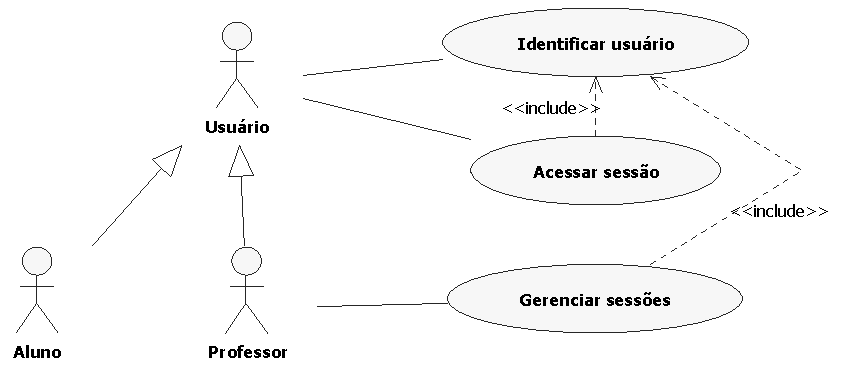
\includegraphics[width=1.0\textwidth]{imgs/img-use-case1.pdf} 
%\caption{Diagrama de casos de uso - identificação e acesso a ferramenta}
%\label{fig:use_case1} 
%\end{figure}

Os casos de uso da Figura \ref{fig:use_case1} mostram o acesso de um usuário que está utilizando a ferramenta como professor. Nela o mesmo pode gerenciar sessões, e gerar todas as informações que são distribuídas a todos os demais usuários.

 

%\begin{figure}[!h]
%\centering
%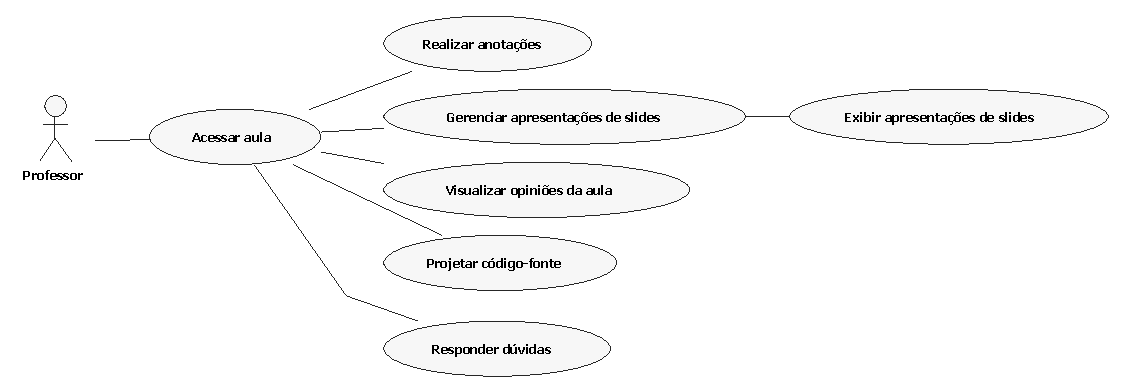
\includegraphics[width=1.0\textwidth]{imgs/img-use-case2.pdf} 
%\caption{Diagrama de casos de uso - acesso como professor}
%\label{fig:use_case2} 
%\end{figure}

A Figura \ref{fig:use_case3} mostra os casos de uso relacionados ao ator aluno. É formado por casos de uso que permitem ao usuário visualizar as informações geradas pelo professor e interagir através de perguntas e do compartilhamento das próprias anotações.

 
%\begin{figure}[!h]
%\centering
%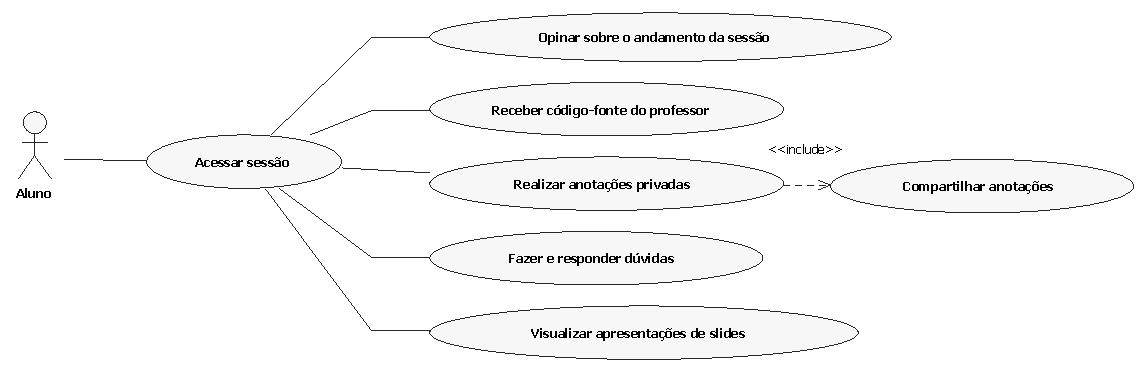
\includegraphics[width=1.0\textwidth]{imgs/img-use-case3.pdf} 
%\caption{Diagrama de casos de uso - acesso como aluno}
%\label{fig:use_case3} 
%\end{figure}

\subsection{Visão de dados}

O diagrama de classes permite a visualização das classes utilizadas pelo sistema e como estas relacionam, permitindo assim uma visão estática de como os dados utilizados na ferramenta são persistidos. O diagrama de classe do projeto é mostrado na Figura \ref{fig:class_diagram}.

 

%\begin{figure}[!h]
%\centering
%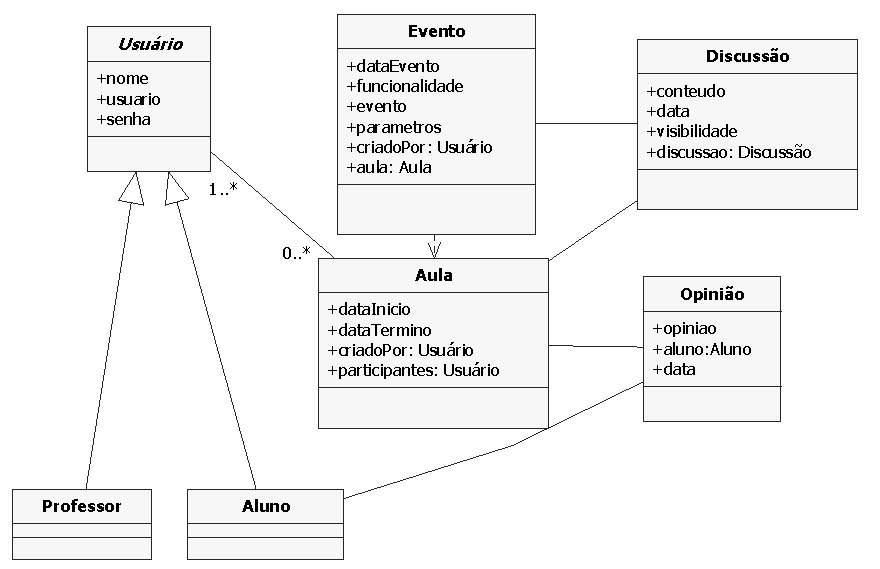
\includegraphics[width=1.0\textwidth]{imgs/img-class-diagram.pdf} 
%\caption{Diagrama de classes}
%\label{fig:class_diagram} 
%\end{figure}

A classe Usuário é abstrata e portanto só pode ser instanciada pela suas sub-classes Aluno e Professor. Estas 3 classes que serão utilizadas para representar os dados dos usuários do sistema. A classe Sessão é um periodo de utilização da ferramenta, ela pode ser criada por um Professor ou por um Outro Sistema através da interface de integração.

A classe Evento é relacionada a todo tipo de ação ou atividade realizada dentro de uma sessão. Por exemplo, uma anotação é um evento. Ela possui um auto-relacionamento, pois em determinadas situações como em dúvidas,  pode estar relacionado a resposta da mesma.

A classe Módulo é responsável pelos dados de todos os módulos da ferramenta. Esta classe e as já descritas acima deverã sofrer alterações até a finalização do projeto para que possa atender a todos os requisitos do projeto. 

\iffalse
\subsection{Padrão de projetos MVC - \emph{model-view-controller}}

No desenvolvimento da ferramenta Mindboard será utilizado o padrão de projeto MVC. Este padrão é definido como um padrão em camadas \cite{pressman} que divide o código em 3 partes, e também define como é a comunicação entre elas.

Ao usuário fazer uma requisição na ferramenta, a mesma é mapeada a um \emph{controller}. O \emph{controller} utiliza o \emph{model} ou os \emph{models} responsáveis por realizar a operação em questão e direciona ao \emph{view} que exibirá a interface de forma apropriada \cite{mvc}. A Figura \ref{fig:mvc} mostra este processo em uma ferramenta web.

\fi



\subsection{Tecnologias}
\label{sec:tecnologias}

Os requisitos não funcionais da ferramenta Mindboard sugerem que a mesma possua uma arquitetura que possa ser escalável. Para atingir este objetivo foram pesquisados formas de disposição de servidores que permitissem a adição de recursos computacionais de forma simples. Foram encontrados alguns estudos de caso e relatos em ferramentas comerciais que possuem um grande número de usuários e como a arquitetura pode ser escalável Sendo assim, a arquitetura proposta para a ferramenta Mindboard foi baseada em relatos de implementações nas ferramentas Box.com \cite{boxcom}, Trello \cite{trello} e Boo-Box \cite{boobox}. A Figura \ref{fig:arquitetura} mostra esta arquitetura.

%\begin{figure}[!h]
%\centering
%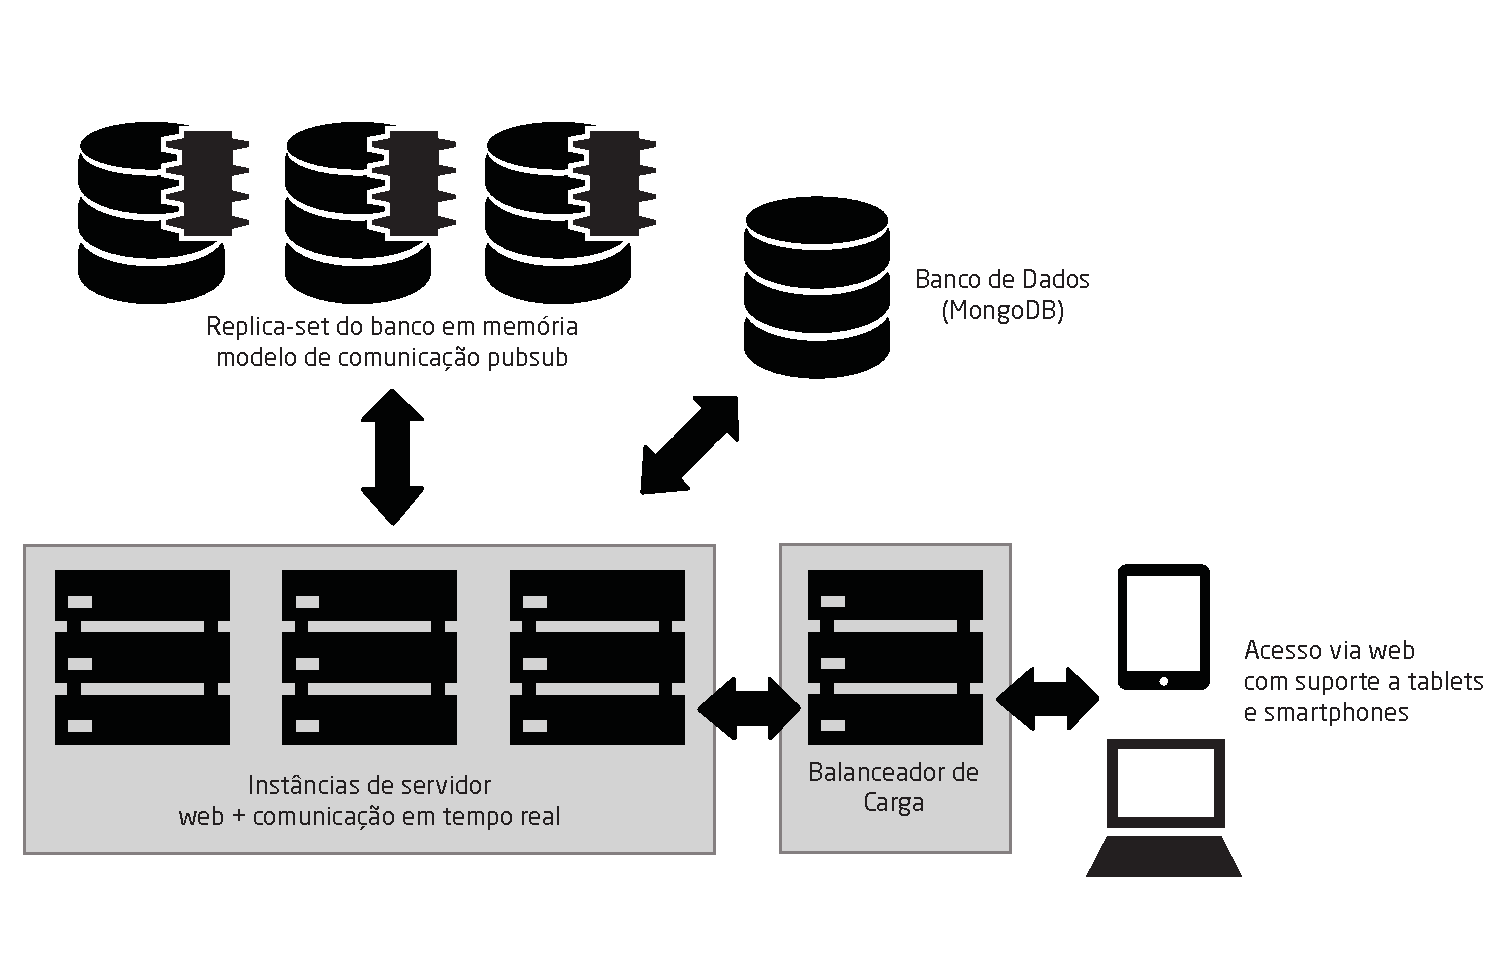
\includegraphics[width=1.0\textwidth]{imgs/img-arquitetura-lb.pdf} 
%\caption{Arquitetura de servidores do Mindboard}
%\label{fig:arquitetura} 
%\end{figure}

O balanceador de carga é composto por um ou mais servidores que recebem as requisições dos usuários e as redistribui em servidores de aplicação. Durante esta redistribuição o balanceador de carga tenta manter a mesma carga em cada um dos servidores de aplicação.

A camada de servidores de aplicação é responsável por receber as requisições do balanceador de carga e processar de forma completa a requisição do usuário. Em algumas situações será necessário ler e persistir dados, neste caso, a aplicação faz esta operação em um dos servidores de banco de dados. A comunicação entre servidores é realizada utilizando o banco em memória.

O banco de dados é configurado como um \emph{replica-set}, ou seja, vários servidores espelhados e que em cada instância da aplicação pode conectar-se e realizar operações. Nesta configuração há a garantia de disponibilidade de dados e também o aumento da performance.

A camada de comunicação entre servidores é composta por instâncias de servidores em memória utilizando o padrão de comunicação \emph{pubsub}. Esta camada é responsável por permitir uma comunicação entre os servidores de forma rápida, pois os dados não são persistidos e são mantidos apenas em memória.

Após a definição da arquitetura, foram definidas quais tecnologias poderiam ser utilizadas em cada uma delas, começando pela interface com o usuário. 

Os requisitos não funcionais da ferramenta Mindboard norteia a utilização de tecnologias para a criação de interfaces que sejam compatíveis com mais de uma plataforma e que possam conter suporte a dispositivos móveis. Sendo assim, após realizada algumas provas de conceito e após o desenvolvimento de ferramentas utilizadas no grupo de pesquisas LiNE, as tecnologias adotadas foram HTML5, CSS 3 e JavaScript.

A tecnologia HTML5 aumentou a padronização no desenvolvimento de aplicações web, principalmente focando em padronizar como utilizar interação entre os elementos \cite{html5}. Visualmente, a interface HTML5 foi formatada utilizando CSS3, que inclusive permite a criação de interfaces responsivas. Já JavaScript permite manipular o HTML5 e principalmente realizar a comunicação em tempo real com o servidor.

O servidor de aplicação foi desenvolvido em JavaScript principalmente para manter uma mesma linguagem no servidor e no cliente. Por este motivo, foi utilizado o NodeJS para a execução do código no servidor.

A tecnologia NodeJS é um ambiente que possibilita a execução de códigos JavaScript no servidor utilizando a mesma tecnologia por trás do Google Chrome, a engine V8 \cite{nodejs}. Uma característica muito importante presente no NodeJS que é fundamental para sistemas de comunicação em tempo real, é o fato do código ser \emph{non-blocking} para operações de entrada e saída, isso permite obter uma boa estabilidade e performance para sistemas que possuem comunicação em tempo real \cite{nodejs}.

Já os dados serão persistidos utilizando o banco de dados MongoDB. O MongoDB é um banco não relacional orientado a documentos. Sua estrutura é baseada em coleções de documentos que podem conter estruturas diversas, sendo assim, uma forma de armazenamento que não possui um \emph{schema} definido \cite{mongodb}. 

É uma forma de armazenar grandes volumes de dados de forma bastante eficiente, e de acordo com \cite{mongodb} o tempo para inserir grandes quantidades de informação chega a ser 15 vezes inferior que a inserção da mesma quantidade de informações em um banco de dados Oracle. O tempo para a realização de outras operações no MongoDB também são bem inferiores se comparado ao Oracle \cite{mongodb}.

O banco em memória Redis \cite{redis_site} é um banco \emph{key-value} que permite a construção de aplicações que utilizam comunicação em tempo real intensamente. Sua arquitetura de uso é bastante flexível, sendo possível criar instâncias replicáveis da mesma. Na arquitetura do Mindboard será utilizada sua funcionalidade \emph{pubsub}.

A funcionalidade \emph{pubsub} \cite{redis_pubsub} permite que sejam criados canais de dados entre instâncias de servidores de aplicações distintos. Um canal de dados é criado, e os usuários que pretendem ser notificados de atualizações de informações naquele canal o fazem através do \emph{subscribe}. Toda vez que uma nova informação é gerada (\emph{publish}), todos os usuários que fizeram um \emph{subscribe} no canal receberão a informação.


O banco em memória possui a velocidade como uma de suas características principais. Estudos de caso como o descrito em \cite{redis_perf} mostram que em uma instância do banco Redis sendo executada em uma máquina Linux 2.6, Intel Xeon X3320 2.5Ghz consegue obter manter um a marca de 110.000 escritas de dados por segundo e 81.000 leituras de dados por segundo.

Esta seção sobre tecnologias ainda sofrerá alterações e atualizações até a finalização do projeto.









        Agradecimentos: 
            - orientador, noiva, familia, pessoal do line, matheus, etc
        Introdução:
            - Falar do passado, que a tecnologia vem evoluindo e mudando como lidamos com ela;
            - O mundo está cada vez mais conectado;
            - As crianças/estudantes estão cada vez mais usando a internet;
            - programas governamentais 
            - ao mesmo tempo do BYOD
                - estudantes se distraem
                - poderiam utilizar alguma ferramenta para comunicar-se em tempo-real;
            - Objetivo (alternativa 1):
                Com base neste contexto, seguintes perguntas de pesquisa:
                    1- Quais seriam as funcionalidades interessantes/relevantes de um sistema colaborativo para ser utilizado dentro e fora de sala de aula?
                    2- Quais seriam as tecnologias adequadas no desenvolvimento de um sistema colaborativo para ser utilizado dentro e fora de sala de aula (levando em conta alguns requisitos)?

                    (juntar com o de cima) 3- Quais seriam as tecnologias adequadas para que pudesse funcionar em mais de uma plataforma e dispositivo?

                    (como forma de teste) 4- Quais os impactos a utilização deste sistema implica em um curso presencial?

                    Hipóteses:
                    para pergunta 1:
                        - se um conjunto de funcionalidades propostas seria o suficiente para ser utilizada, seria avaliado com a pesquisa, literatura e experimento

                        - que as funcionalidades seriam x,y,z
                            - para validar esta hipótese, foi conduzida uma pesquisa com professores e alunos, feita revisão da literatura, 
                        - content-sharing: construção de conteúdo > code-sharing > text-sharing > equações (latex ou tex)

                    para pergunta 2:
                        - Hipótese 1:
                            - tais tecnologias são boas utilizar HTML 5, ...

                            - Alternativa 2:
                                - utilizar java applet (vai ser desconsiderado, de acordo com os testes que fiz no LiNE), perguntar se pode usar pro Leo - gostaria de descrever o experimento
                                - Chrome está reduzindo o suporte:
                                    https://java.com/en/download/faq/chrome.xml

                    (como experimento - objetivo secundário):
                        - hipótese 1:
                            - uma ferramenta com as características definidas ajuda na condução e no aprendizado em um curso presencial:
                            - para validar:
                                - curso presencial com a pesquisa dos alunos depois

            - objetivo:
                - testar / verificar / pesquisar

            - estrutura do documento (este capitulo falou disso, o proximo disso , blablabla)

            /*- LEMBRAR da intro do danilo históricozinho


            - Objetivo (alternativa 2):
                - falar das projetar e desenvolver uma ferramenta tal e tal
                - que permitisse colaboração

                - justificativa:
                    - experiência minha como professor de programação, onde tinha que compartilhar código e etc,
                    - percebi que este processo poderia ser melhorado;*/

        2 - Fundamentos:
        para cumprir os objetivos do capitulo 1, este trabalho vai lidar com varios conceitos da area da educacao, colaboracao e etc, aqui serao discutidos os conceitos blablabla, 
            - como começou informatica na educação que deu origem a blablabla
            - Aprendizado mediado por computador ou aided
            - Aprendizado colaborativo:
                - História que começa a colaboração com CSCW, no ambiente de trabalho. Groupware, evolui para CSCL. A colaboração pode ser utilizada com várias finalidades:
                    - Planejamento das aulas;
                    - Condução das aulas;
                    - Atividades extra-classe e etc;
                - CSCW / CSCL
                    - nosso sistema vai ser colaborativo, para ser um sistema colaborativo nós precisamos conhecer as características e discutir bastante cada uma delas... mais de uma página para cada um destes itens. basear em mais de um artigo e livros bases; contrastar, discutir, etc, biased...
                    - características relevantes para um sistema CSCL
                        - visibilidade (artigo: Using online collaboration applications for group assignments- The interplay between design and human characteristics.pdf);
                    - como o usuário pode definir quem pode acessar aquela informação;
                    - detalhe que o usuário pode fazer com mais vontade quando a info vai ser vista por mais gente e não só o professor;
                        - Comunicação em sala de aula: 
                            - síncrona 
                            - assíncrona;
            - LMS:
                - História dos primeiros LMSs até chegar a falar do moodle que é um dos mais famosos e utilizados;
            - Sincronismo entre os pontos e Operational transformation
                - Arquitetura de rede, servidor centralizado (pq?)
                - a forma de pensar mais simples sobre como sincronizar, seria a cada alteração, enviar todas as informações para todos os nós envolvidos;
                (fazer grafico e mostrar estimativa de quanto seria transferido de um ponto ao outro)
                    - porem isso gera um problema: 
                        - grande número de informações trocadas;
                        - incosistência caso duas informações cheguem ao servidor ao mesmo tempo;


        3 - Metodologia (TALVEZ INTRODUÇÃO) - explicar o COMO:
            - explica tudo sem gráfica, a figura x no fim, ilustra um resumo do processo... Processo, gráfico
            - revisão, da revisão exploratoria e da outra, foi confirmado o conjunto de funcionalidades, então foi feita pesquisa com professore e alunos, aceitariam isso (SEM FALAR de resultados)
                - COMO foi feita (pela internet, )
                - riscos a validade (foi feita pela internet), no entanto é o público alvo
                - pesquisa como anexo
            - experimento do line
            - experimento, falar dele... talvez resumo, e no capitulo x vai ser explicado o experimento com mais detalhes (qual curso, etc)



        4 - Revisão da literatura: revisão sobre sistemas de apoio ao ensino / características de sistemas de aprendizado:
            - Foi conduziada uma revisão exploratória da literatura, onde o processo de obtenção de dados seguiu uma pequena metodologia, porém, está metodologia não foi tão rígida a ponto de ser considerada uma revisão sistemática;
            - Levantamento dos requisitos disponíveis nos sistemas e tal;
            - Conhecer os sistemas utilizados no mercado e em artigos;
        

        5 - Resultados da pesquisa alunos professores
        
        6 - Tecnologias:
                - resultado da pesquisa com o line
                - arquitetura: Boo-Box
                - tecnologias


        7 - Mindboard:
            - discussão das features sugeridas
            - projeto e implementação do sistema Mindboard:
                - Processo Unificado customizado por bernardes
                    - descrição das iterações - historinha () - gerar artefatos
                - 4.3.1 - Descricao dos requerimentos
                - requisitos funcionais
                - requisitos não-funcionais
                    - como artefato: lista sem discussão
                    - responsivo
                - diagramas de classe
                    - adaptado para modulo
                - diagramas de estado
                - GLOSSÁRIO de TERMOS usados na ferramenta:
                    - aula
                    - projeção de conteúdo
                    - etc...
                - esboço da interface
                    - mock em papel
                    - responsivo -- ligado
                - casos de uso alto nível
                    - descrever anexo
                - img 21 - dissertacao do joao - diagrama de subsistemas (mestrado do joao)
                - UML alto nível (das caixinhas se preciso ou só texto)
                    - explicar bem explicado
                - diagrama de estado
                    - 
                - implementação e testes (ligação pro )
                    - visão geral do sistema,
                    - no fim o sistema ficou assim
                    - implementou de tal jeito
                    - pequenos testes durante o desenvolvimento
                    - no final com testes mais específicos
            - Implementação


        8 - Teste:
            - contar historinha, processo do CEP (aquele doc que mandei pro CEP)
            - tudo que tem no doc do cep coloca aqui, o q tem e já foi falado falar resumido;
            - ajustar coisas que eu ia medir interacoes
                - log
                - video
                - perguntando
                - nos resultados, na contagem tivemos problemas x, y e z.
            - citar o num do experimento no CEP e como foi conduzido
            - formulário USE
            - fotos do ambiente
                - como foi contada cada interação pelo vídeo
            - experimento nao foi bom, por poucos alunos
                - grupo controle usou mto o fb
                - favorece interação pessoal,
                - amigos
                - each
                - o cara isolado
                - tentar estimar % das interações com dúvidas no código; 
                    - revisar contagens - se for uns 10%
                - como foi contado;

        ==================================================================

        9 - Resultados e discussões:
            - Interações:
                - contadas nos vídeos
                - contadas nos logs
            - Uso de recursos como code-sharing
            - Uso de recursos como o like/disliking
            - Flipped classroom e aulas de programação
            - Code-sharing
            - Questionário USE

        Conclusões:
            - Comparar cada pergunta de pesquisa, e qual hipótese foi confirmada ou invalidada
            - Trabalhos futuros:
                - resultados da pesquisa por questão de tempo e escopo, num trabalho futuro, 2 turmas grandes, pelo mesmo professor, num ambiente sala de aula, onde os alunos podem usar os dispositivos, sem o professor ser o mesmo pesquisador, se não aumentou, investigar o pq
                - Integrar IDE com o code-sharing do mindboard
                - Divisão dos códigos projetados em projetos
                - Rever a criação do projeto
                - Permitir colaboração

        03/04/2015 - reunião


